% This is part of Un soupçon de mathématique sans être agressif pour autant
% Copyright (c) 2012
%   Laurent Claessens
% See the file fdl-1.3.txt for copying conditions.

\begin{exercice}\label{exoSeconde-0069}

    \begin{multicols}{2}

À partir du graphique ci-contre, répondre par vrai ou faux aux affirmations suivantes.

\begin{enumerate}
    \item
       L'image de \( 1\) par la fonction \( f\) est \( 0\).
   \item
       L'image de \( 0\) par la fonction \( f\) est \( 1\).
   \item
       L'image de \( 7\) par la fonction \( f\) est \( 4\).
   \item
       Les antécédents de \( 3\) sont \( 2\) et \( 4\)
   \item
       \( f(3)=4\).
   \item
       \( f(2)=5\).
   \item
       \( f(3)>f(5)\).
   \item
       \( f\) est croissante sur \( \mathopen[ 1 , 3 \mathclose]\).
   \item
       \( f\) est décroissante sur \( \mathopen[ 3 , 6 \mathclose]\).
    \item
        \( f\) a un minimum pour \( x=5\) et il vaut \( 2\).

\end{enumerate}
Source : \cite{BPizfV}.

\columnbreak


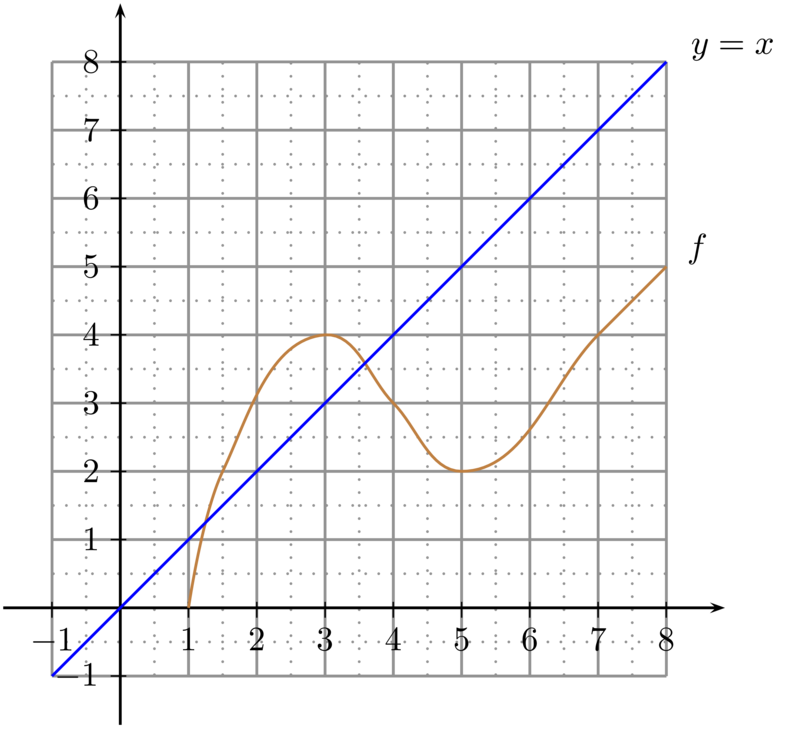
\includegraphics{Picture_FIGLabelFigExoIntersectionCourbenzIxXdPICTExoIntersectionCourbenzIxXd-for_eps.pdf}

    \end{multicols}

Toujours à partir du même dessin, donner les solutions (approximatives) de l'équation \( f(x)=x\) et résoudre l'inéquation
\begin{equation}
    f(x)\geq x.
\end{equation}

\corrref{Seconde-0069}
\end{exercice}
